\section{Medición empírica}

Para comprobar empíricamente la complejidad \textbf{O($n^2$)} del algoritmo, se decidió ejecutar el mismo con distintos tamaños de entrada y medir el tiempo de ejecución. Se generaron muestras de tamaño n, las cuales varían desde 10 hasta 1000.

Para cada muestra se registró el tiempo de ejecución, obteniendo el siguiente gráfico:

\begin{center}
    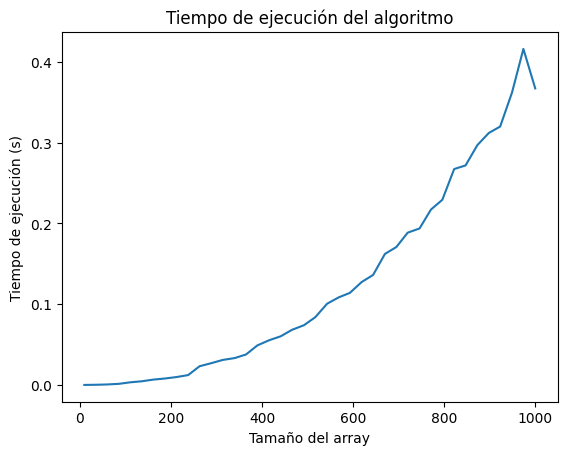
\includegraphics[scale = 0.6]{ {images/image.png} }
\end{center}


A simple vista se puede observar un crecimiento cuadratico. Para confirmar esto, vamos a ajustar los datos a una recta mediante cuadrados mínimos. Esto lo realizamos con Python y la función \textit{optimize.curve\_fit} de la biblioteca \textit{scipy}.


Obtenemos que el gráfico se puede ajustar a la curva $y = 4.86e^{-07}x^{2} -9.84e^{-05}x + 0.007$, con un error cuadrático medio de $9.37e^{-05}$. Por lo tanto, podemos verificar lo que ya vimos en la sección 3, que el orden es cuadratico \textbf{O($n^2$)}.

\begin{center}
    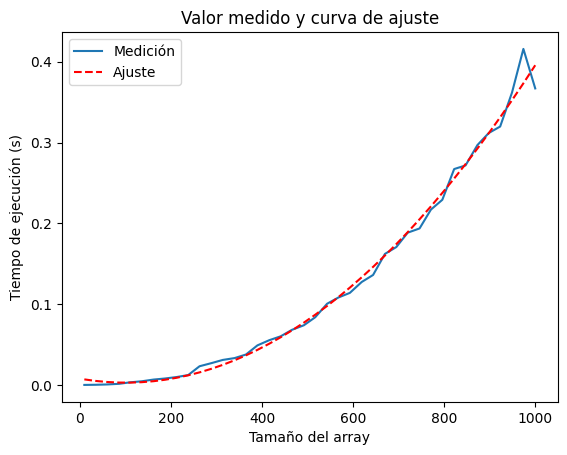
\includegraphics[scale = 0.6]{ {images/cuadradosMinimos.png} } 
\end{center}